\section{Experiments}
\label{sec:exp}

\subsection{Protocol}
\label{sec:exp:protocol}

\paragraph{Setup.} All arms fine-tune SD3.5-Medium with LoRA under an identical
$100$-optimizer-update budget, the same composite reward
($\textsc{PickScore}+\textsc{CLIP}+\textsc{HPSv2}$ on raw scores), the same data
($1152$ samples/epoch from Pick-a-Pic), $512^2$ resolution and guidance scale $1.0$.
An arm and its baseline always share \emph{training hardware, world size, random seed, and
outer epoch}; we verified that mismatching any of these produces artifacts of the same
order as the effects we report (App.~\ref{app:pairing}).

\paragraph{Evaluation.} We report the composite $\textsc{Pick}/26+\textsc{CLIP}+\textsc{HPSv2}$
on two prompt sets -- DrawBench ($200$ unique prompts $\times5$ images) and
\emph{Unseen-1k} ($1000$ unique held-out Pick-a-Pic prompts) -- generated with the
rectified-flow sampler at $\mathrm{NFE}\in\{2,4,6,10,20,40\}$, always on A40 GPUs, with
$n\!=\!1000$ images per cell. Differences are per-image paired and reported in units of
$\mathrm{MDE}=0.0033$.

\paragraph{What counts as an effect.} Effect sizes in this literature are often comparable
to run-to-run variation, so we measured the variation directly: across $8$ unmodified
canonical arms (differing only in hardware, world size or seed) the $28$ pairwise
differences have median $|\Delta|=0.39$ MDE and maximum $1.23$ MDE; two runs of the
\emph{identical} configuration differ by $0.56$ MDE (App.~\ref{app:floor}). We therefore
require $|\Delta|\ge2.5$ MDE with $t>2$ for a single-seed claim, or $1$--$2.5$ MDE with a
same-signed second seed.

\paragraph{Held-out evaluator.} Across $12$ arms spanning $-35$ to $+18$ MDE, ImageReward
tracks the reported composite ($r=+0.894$, sign agreement $12/12$) whereas Aesthetic is
\emph{anti}-correlated ($r=-0.395$, $4/12$). We therefore report ImageReward as the
held-out evaluator and do not report Aesthetic (App.~\ref{app:evalcal}).

\subsection{Reproduction fidelity}
\label{sec:exp:repro}

Before any comparison we check that our reproduction and our evaluation agree with the
published protocol. We match it on every axis we could verify: LoRA rank $32$ and alpha
$64$ at $512^2$, Pick-a-Pic training prompts, CFG-free rollouts with guidance $1.0$ and a
deterministic $10$-step DPM-Solver++ 2M, $48$ prompt groups of $24$ images per optimizer
update, AdamW at $3\times10^{-4}$, trust region $\rho=0.10$, two target steps,
branch coefficient $\beta=0.1$ for the joint three-reward objective and $1.0$ for
reward-specific runs, checkpoint-averaged parameters at save time, and DrawBench
evaluation with $40$-step flow sampling at guidance $1.0$.

Table~\ref{tab:official} puts the two side by side. The untrained base model -- which
involves no training code at all, and therefore isolates the evaluation pipeline -- agrees
with the published numbers to $0.4\%$ on PickScore, $1.6\%$ on CLIPScore, $1.5\%$ on
HPSv2.1 and $0.1\%$ on Aesthetic. That row is marked in the source as partly inherited from
an earlier report rather than re-measured, so we treat it as a check on the protocol rather
than on any one group's measurement.

\paragraph{The joint objective at the published budget.} Trained for the published $300$
updates, our reproduction lands within the measurement tolerance on \emph{all five}
evaluators:

\begin{center}
\begin{tabular}{lccccc}
\toprule
& Pick & CLIP & HPSv2.1 & Aes & ImgR\\
\midrule
reported \citep{opsd2026} & $25.51$ & $0.333$ & $0.389$ & $6.03$ & $1.51$\\
ours, $300$ updates       & $25.46$ & $0.332$ & $0.388$ & $5.95$ & $1.51$\\
\midrule
$|\Delta|$ as a fraction of tolerance & $0.12$ & $0.21$ & $0.19$ & $0.81$ & $0.11$\\
\bottomrule
\end{tabular}
\end{center}

The tolerance is not chosen after the fact: it is the $1.6\%$ agreement measured on the
untrained backbone above, which bounds what the evaluation pipeline alone can account for,
and seven unmodified canonical runs spanning three GPU types, two world sizes and two seeds
vary by at most $0.65$ of that tolerance on any column (App.~\ref{app:floor}). Our numbers
are consistently a touch below the published ones, but the largest gap is $0.81$ of the
tolerance and the median is $0.19$, so the offset is not separable from the pipeline itself.
We therefore read the published method as reproduced at its own budget, and report the
baselines it is compared against as inherited rather than re-measured.

Table~\ref{tab:official} also carries the baselines reported alongside \opsd. We did not
rerun them; the upper block is reproduced from that paper so that our numbers can be read
against the same field, and we mark it as such rather than presenting it as our
measurement. One entry is worth noting even at this stage: at $100$ updates \MSP already
reaches the ImageReward value that \opsd reports at $300$ ($1.51$), and exceeds every
non-\opsd baseline in that column, including DiffusionNFT at $300$ updates ($1.45$) and
FlowGRPO at $4$k ($1.29$). That value also matches our \emph{own} canonical run at the
full $300$ updates ($1.5066$), so the comparison does not depend on reading across
laboratories. \MSP at $100$ updates remains below the $300$-update row on the three
components of the training composite, which is what a third of the budget should give, so
this is an observation about the held-out column and not a claim that a third of the budget
suffices; the matched $300$-update \MSP run is still training.

The stronger check is a \emph{trained} checkpoint, and here the published numbers are ones
the original authors measured themselves rather than inherited. The reward-specific block is
trained under a different recipe from the joint one --- $100$ updates and $\beta=1.0$ rather
than $300$ and $0.1$ --- so it is an independent test of the same code. Reproducing it gives
HPSv2.1 $0.3920$ against a reported $0.390$ ($0.5\%$) and PickScore $24.96$ against $24.94$
($0.08\%$). The CLIPScore column is the one place our reproduction falls outside that
tolerance: $0.3203$ against a reported $0.340$, a gap of $5.9\%$. The evaluator is not the
cause --- our CLIPScore agrees with the published value to $1.6\%$ on the untrained backbone
and to $0.33\%$ on the joint $300$-update row --- so the gap is specific to the
CLIPScore-trained run, which is still improving when its budget ends. We report it rather
than tune towards it (App.~\ref{app:rewardspec}); the two remaining columns are not yet
available.
Those numbers exercise the training code, the target construction and the evaluation
together, and their deviations run in the opposite direction from the joint block's, so
there is no systematic offset. We take the reproduction as verified rather than assumed.

We also checked that one published hyper-parameter is not arbitrary. The protocol sets the
branch coefficient to $\beta=0.1$ for the joint objective; retraining the canonical arm at
$\beta=1.0$ and changing nothing else costs it $5.09$ and $6.09$ MDE on DrawBench at $4$ and
$40$ steps, and $5.45$ and $6.02$ on the held-out prompt set, with per-image win rates of
$20$--$27\%$. The published value is therefore tightly tuned for this objective. (That arm
ran on a different accelerator from its control; the offset such a swap induces is
$\le0.55$ MDE, App.~\ref{app:pairing}, against an effect of $5$--$6$.)

% 自动生成,勿手改。源:paper_figs/make_table_official.py
\begin{table}[t]
\centering
\setlength{\tabcolsep}{4pt}
\caption{\textbf{SD3.5-M under the published protocol.} DrawBench, $40$-step flow,
guidance $1.0$, $512^2$, $n{=}1000$, checkpoint-averaged parameters. The upper block is
reproduced verbatim from \citet{opsd2026}; we did not rerun those baselines. The lower
block is ours under the same protocol. \cmark: one checkpoint per evaluator column;
\xmark: a single checkpoint evaluated across all columns. Higher is better.}
\label{tab:official}
\resizebox{0.98\linewidth}{!}{%
\begin{tabular}{lcc rrrrr}
\toprule
\textbf{Model} & \textbf{R.-spec.} & \textbf{Upd.} & \textbf{Pick} & \textbf{CLIP} & \textbf{HPSv2.1} & \textbf{Aes} & \textbf{ImgR}\\
\midrule
\multicolumn{8}{l}{\textbf{Reported by \citet{opsd2026}}}\\
\midrule
\multicolumn{8}{l}{\emph{Reference backbones}}\\
\quad SDXL & \xmark & -- & $22.42$ & $0.287$ & $0.280$ & $5.60$ & $0.76$\\
\quad SD3.5-L & \xmark & -- & $22.91$ & $0.289$ & $0.288$ & $5.50$ & $0.96$\\
\quad FLUX.1-dev & \xmark & -- & $22.84$ & $0.295$ & $0.274$ & $5.71$ & $0.96$\\
\midrule
\multicolumn{8}{l}{\emph{SD3.5-M, one checkpoint across all columns}}\\
\quad SD3.5-M w/o CFG & \xmark & -- & $20.51$ & $0.237$ & $0.204$ & $5.13$ & $-0.58$\\
\quad $+$ CFG & \xmark & -- & $22.34$ & $0.285$ & $0.279$ & $5.36$ & $0.85$\\
\quad $+$ FlowGRPO & \xmark & 4k & $23.50$ & $0.280$ & $0.316$ & $5.90$ & $1.29$\\
\quad $+$ DiffusionNFT & \xmark & 300 & $23.62$ & $0.294$ & $0.340$ & $6.02$ & $1.45$\\
\quad $+$ DanceOPD & \xmark & 300 & $23.06$ & $0.272$ & $0.322$ & $5.98$ & $1.23$\\
\quad $+$ DiffusionOPD & \xmark & 300 & $23.05$ & $0.269$ & $0.322$ & $6.04$ & $1.23$\\
\quad $+$ FlowOPD & \xmark & 300 & $22.62$ & $0.263$ & $0.300$ & $5.98$ & $0.92$\\
\quad $+$ \opsd & \xmark & 300 & $25.51$ & $0.333$ & $0.389$ & $6.03$ & $1.51$\\
\midrule
\multicolumn{8}{l}{\emph{SD3.5-M, one checkpoint per evaluator}}\\
\quad $+$ ReFL & \cmark & 100 & $23.92$ & $0.308$ & $0.358$ & $12.09$ & $1.28$\\
\quad $+$ DiffusionNFT & \cmark & 100 & $23.43$ & $0.298$ & $0.336$ & $9.11$ & $1.46$\\
\quad $+$ \opsd & \cmark & 100 & $24.94$ & $0.340$ & $0.390$ & $12.08$ & $1.76$\\
\midrule
\multicolumn{8}{l}{\textbf{Ours, same protocol}}\\
\midrule
\quad SD3.5-M w/o CFG & \xmark & -- & $20.59$ & $0.241$ & $0.207$ & $5.12$ & $-0.55$\\
\quad $+$ \opsd (repro) & \xmark & 100 & $24.66$ & $0.316$ & $0.370$ & $5.90$ & $1.43$\\
\quad $+$ \opsd (repro) & \xmark & 300 & $25.46$ & $0.332$ & $0.388$ & $5.95$ & $1.51$\\
\quad $+$ \MSP (ours) & \xmark & 100 & $24.84$ & $0.323$ & $0.376$ & $5.94$ & $1.51$\\
\quad $+$ \MSP (ours) & \xmark & 300 & $25.11$ & $0.327$ & $0.376$ & $5.94$ & $1.41$\\
\midrule
\multicolumn{8}{l}{\emph{SD3.5-M, one checkpoint per evaluator}}\\
\quad $+$ \opsd (repro) & \cmark & 100 & $24.96$ & $0.320$ & $0.392$ & $12.18$ & $1.76$\\
\quad $+$ \MSP (ours) & \cmark & 100 & $24.95$ & $0.319$ & $0.391$ & $9.47$ & $1.79$\\
\bottomrule
\end{tabular}}
\end{table}


\subsection{Main results}
\label{sec:exp:main}

% 主表 — 自动生成,勿手改。源:paper_figs/make_table_main.py
\begin{table}[t]
\centering
\setlength{\tabcolsep}{3.5pt}
\caption{\textbf{Main results on DrawBench} (SD3.5-Medium, $100$ optimizer updates, A40 eval,
$n{=}1000$ prompts). Absolute scores; \textbf{bold}: best, \underline{underline}: second best.
Composite $=$ PickScore$/26+$CLIP$+$HPSv2 is the reported metric; ImageReward is the held-out
evaluator and is never trained on. Rows marked ``--'' are baselines we have not run yet.
The (A) row was trained on $3$ processes rather than $4$; the offset this induces is $0.17$ MDE
(App.~\ref{app:pairing}).}
\label{tab:main}
\resizebox{0.98\linewidth}{!}{%
\begin{tabular}{l ccccc ccccc}
\toprule
& \multicolumn{5}{c}{\textbf{NFE}$=$\textbf{4}} & \multicolumn{5}{c}{\textbf{NFE}$=$\textbf{40}} \\
\cmidrule(lr){2-6}\cmidrule(lr){7-11}
\textbf{Method} & \textbf{PickScore} & \textbf{CLIP} & \textbf{HPSv2} & \textbf{Composite} & \textbf{ImageReward} & \textbf{PickScore} & \textbf{CLIP} & \textbf{HPSv2} & \textbf{Composite} & \textbf{ImageReward} \\
\midrule
SD3.5-M (no reward training) & 19.64 & 0.2170 & 0.1343 & 1.1069 & -1.705 & 20.59 & 0.2408 & 0.2070 & 1.2396 & -0.548 \\
\quad + SFT on teacher rollouts & -- & -- & -- & -- & -- & -- & -- & -- & -- & -- \\
\quad + few-step distillation (DMD2/TDM) & -- & -- & -- & -- & -- & -- & -- & -- & -- & -- \\
\midrule
\quad + OPSD \citep{opsd2026} \emph{(prior SOTA)} & 23.97 & 0.3100 & 0.3413 & 1.5732 & 1.304 & 24.66 & 0.3165 & 0.3704 & 1.6353 & 1.433 \\
\quad\quad (A) query $\sigma$ 0.278$\to$0.465 & \underline{24.40} & 0.3189 & \underline{0.3592} & \underline{1.6166} & 1.416 & 24.67 & 0.3164 & 0.3685 & 1.6337 & 1.460 \\
\quad\quad (B) rollout 10$\to$6 & 24.39 & 0.3167 & 0.3591 & 1.6138 & 1.404 & 24.70 & 0.3149 & 0.3701 & 1.6351 & 1.458 \\
\quad\quad \textbf{(C) $+$ \MSP (ours)} & 24.26 & \underline{0.3208} & 0.3547 & 1.6085 & \underline{1.435} & \textbf{24.84} & \textbf{0.3228} & \textbf{0.3758} & \textbf{1.6538} & \textbf{1.507} \\
\quad\quad (B$+$C) & \textbf{24.53} & \textbf{0.3212} & \textbf{0.3621} & \textbf{1.6268} & \textbf{1.456} & \underline{24.77} & \underline{0.3183} & \underline{0.3717} & \underline{1.6427} & \underline{1.469} \\
\bottomrule
\end{tabular}}
\end{table}


Table~\ref{tab:main} reports absolute scores. \MSP is the best configuration at the full
budget on every axis we report -- composite $1.6538$ and held-out ImageReward $1.5072$ --
and at $4$ steps it already reaches $98.4\%$ of the composite that \opsd attains with
$40$ network evaluations ($1.6085$ vs.\ $1.6353$) -- a $10\times$ reduction in sampling
cost for a $1.6\%$ shortfall. Combining \MSP with a shortened rollout is stronger still at
$4$ steps, taking every axis in the table.

\paragraph{What is the gain worth in training budget?} Our $300$-update reproduction gives
a second reading of the same effect. Within that single run, going from $100$ to $300$
updates --- three times the training compute --- is worth $+15.92$ MDE at four steps on
DrawBench and $+16.65$ on Unseen-1k. Propagation, at $1.21\times$ the cost of a $100$-update
run, is worth $+10.70$ and $+8.20$ on the same cells:

\begin{center}
\begin{tabular}{lcccc}
\toprule
& \multicolumn{2}{c}{DrawBench} & \multicolumn{2}{c}{Unseen-1k}\\
\cmidrule(lr){2-3}\cmidrule(lr){4-5}
& NFE$=4$ & $40$ & NFE$=4$ & $40$\\
\midrule
$3\times$ the training budget ($100\!\to\!300$) & $+15.92$ & $+19.11$ & $+16.65$ & $+22.27$\\
propagation at $100$ updates & $+10.70$ & $+5.62$ & $+8.20$ & $+3.34$\\
\midrule
fraction of the budget increase & $\mathbf{67\%}$ & $29\%$ & $\mathbf{49\%}$ & $15\%$\\
per unit of extra training compute & $\mathbf{6.4\times}$ & $2.8\times$ & $\mathbf{4.7\times}$ & $1.4\times$\\
\bottomrule
\end{tabular}
\end{center}

At four steps propagation recovers half to two thirds of what tripling the budget buys,
for a tenth of the extra compute --- and the ratio is largest exactly where the method is
claimed to act. This is a statement about \emph{marginal} return from $100$ updates: \MSP at
$100$ updates does not overtake the canonical run at $300$ in absolute terms, and the
marginal value of budget is itself budget-dependent, so the conversion should not be
extrapolated beyond this range. The $1.21\times$ figure is measured on two accelerators
(App.~\ref{app:cost}), and the $100$-update checkpoint of the $300$-update run matches the
separately trained $100$-update arm to within the measured floor ($\le0.32$ MDE,
$|t|\le1.35$), so the comparison carries no cross-run confound.

\paragraph{Budget makes the problem worse, not better.} The same $300$-update run also
settles whether the few-step shortfall is simply undertraining. Measuring each model against
\emph{itself} --- its $40$-step score minus its $4$-step score --- the canonical procedure's
deficit grows monotonically with training, from $12.4$ MDE at $20$ updates to $18.8$ at
$100$ and $22.3$ at the published $300$ (DrawBench; $12.0$, $17.3$ and $22.7$ on Unseen-1k).
Extra budget improves the full-budget sample faster than the short one, so the two pull
apart. Propagation moves the curve down at every checkpoint we measured, by $2.1$ to $5.2$
MDE (Fig.~\ref{fig:deficit}). Training longer is not a substitute for changing where the
target is applied; it is what makes the change necessary.

\begin{figure}[h]
\centering
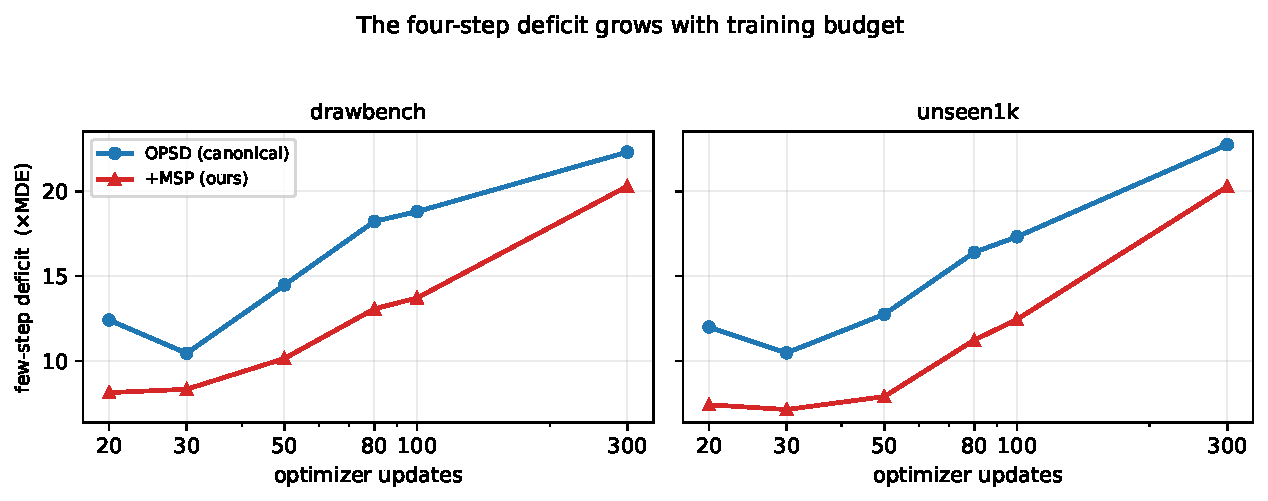
\includegraphics[width=\linewidth]{fig10_deficit_vs_budget.pdf}
\caption{\textbf{The four-step deficit grows with training budget.} Each point is one model
measured against itself: its $40$-step score minus its $4$-step score, paired over $1000$
images. Higher is worse. The canonical curve rises throughout; propagation sits below it at
every checkpoint. The dip at $30$ updates appears on both prompt sets and both arms, so it
belongs to the training trajectory rather than to evaluation noise. The $300$-update point
for propagation is still training and is omitted rather than estimated.}
\label{fig:deficit}
\end{figure}

\begin{figure}[t]
\centering
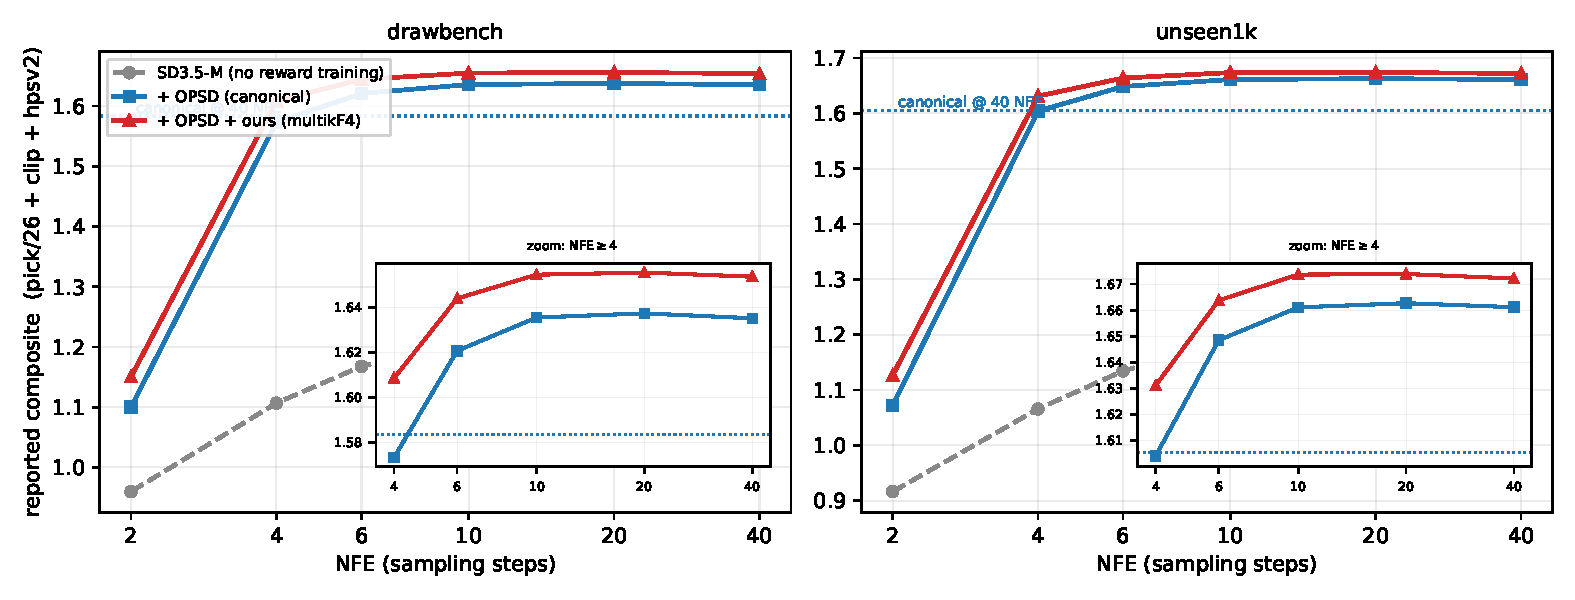
\includegraphics[width=\linewidth]{fig2_quality_vs_nfe.pdf}
\caption{\textbf{Absolute quality versus sampling budget}, both prompt sets. Dotted line:
\opsd evaluated with $40$ steps. On the measured grid \MSP crosses that line at $6$ steps
($5.4$ by interpolation); \opsd itself needs $10$.}
\label{fig:quality}
\end{figure}

\subsection{Where should the target be applied?}
\label{sec:exp:where}

% Table 1 — 自动生成,勿手改。源:paper_figs/make_table1.py
% 口径:SD3.5-M,100 optimizer updates,A40,逐图配对 n=1000/格,MDE=0.0033
\begin{table}[t]
\centering
\setlength{\tabcolsep}{4pt}
\caption{\textbf{Where should the on-policy reward target be applied?} Paired per-image gain over
the canonical OPSD model trained at the \emph{same} budget and on the \emph{same} hardware,
in units of MDE$=0.0033$; win\% in parentheses. A cell counts as a gain when it clears
$2.5\times$MDE with $t>2$, the threshold calibrated against the measured canonical-versus-canonical
noise floor (Sec.~\ref{sec:exp:protocol}); $^\dagger$ marks the $1$--$2.5\times$MDE band, which a single
seed cannot resolve. The last column counts cells that clear the threshold: propagation is the only
\emph{placement} positive at every budget on both prompt sets. The final row is a \emph{reference},
not a placement choice and not a matched-budget comparison: it is the same run read at $300$
rather than $100$ updates, included because tripling the budget is the obvious alternative. It
gains more in absolute terms, at $3.00\times$ the cost; Sec.~\ref{sec:exp:main} gives the
per-unit-compute comparison and Fig.~\ref{fig:deficit} shows that it \emph{widens} the
few-step gap that propagation narrows.}
\label{tab:where}
\resizebox{0.98\linewidth}{!}{%
\begin{tabular}{lcc cc cc c}
\toprule
& & & \multicolumn{2}{c}{\textbf{DrawBench}} & \multicolumn{2}{c}{\textbf{Unseen-1k}} & \\
\cmidrule(lr){4-5}\cmidrule(lr){6-7}
\textbf{Intervention} & \textbf{Cost} & \textbf{Setting} & NFE$=$4 & NFE$=$40 & NFE$=$4 & NFE$=$40 & \textbf{Gains} \\
\midrule
(A) move query state $\sigma$ 0.278$\to$0.465 & $1.00\times$ & \scriptsize ck100, np3 & $+12.71$ \scriptsize(89\%) & $-0.32$ \scriptsize(47\%) & $+13.18$ \scriptsize(94\%) & $-1.09$ \scriptsize(42\%) & $2/4$ \\
(B) shorten rollout 10$\to$6 steps & $0.90\times$ & \scriptsize ck100, np4 & $+12.30$ \scriptsize(91\%) & $-0.05$ \scriptsize(48\%) & $+12.43$ \scriptsize(94\%) & $-0.98$ \scriptsize(43\%) & $2/4$ \\
(C) propagate target to 2 extra states (ours) & $1.20\times$ & \scriptsize ck100, np4 & $+10.70$ \scriptsize(83\%) & $+5.62$ \scriptsize(71\%) & $+8.20$ \scriptsize(80\%) & $+3.34$ \scriptsize(64\%) & $\mathbf{4/4}$ \\
(B$+$C) rollout 6 $+$ propagation & $\sim\!1.10\times$ & \scriptsize ck100, np4 & $+16.23$ \scriptsize(93\%) & $+2.26^{\dagger}$ \scriptsize(56\%) & $+15.91$ \scriptsize(95\%) & $+1.45^{\dagger}$ \scriptsize(54\%) & $2/4$ \\
(A$+$C) query $\sigma$ 0.465 $+$ propagation & $1.20\times$ & \scriptsize ck100, np4 & $+17.00$ \scriptsize(94\%) & $+2.14^{\dagger}$ \scriptsize(57\%) & $+15.32$ \scriptsize(93\%) & $+0.70$ \scriptsize(52\%) & $2/4$ \\
\midrule
\;\emph{(reference)} train $3\times$ longer & $3.00\times$ & \scriptsize ck300 vs ck100, np4 & $+15.92$ \scriptsize(92\%) & $+19.11$ \scriptsize(95\%) & $+16.65$ \scriptsize(94\%) & $+22.27$ \scriptsize(98\%) & $\mathbf{4/4}$ \\
\bottomrule
\end{tabular}}
\end{table}


Table~\ref{tab:where} isolates \emph{where} the gain comes from. Three observations.

\textbf{(A) and (B) are the same intervention.} Moving the query state
($\sigma^\star\!:\,0.278\!\to\!0.465$) and shortening the rollout ($10\!\to\!6$ steps)
agree cell-by-cell: $+12.71$ vs.\ $+12.30$ and $+13.18$ vs.\ $+12.43$ at $4$ steps,
$-0.32$ vs.\ $-0.05$ and $-1.09$ vs.\ $-0.98$ at $40$ steps. This is expected: a $6$-step
schedule has no state near $\sigma\!=\!0.278$, so its nearest-$\sigma$ query lands at
$\sigma_q=0.432$. Shortening the rollout \emph{is} moving the query state.

\textbf{Both are a trade.} Their few-step gains are the largest single-intervention
numbers in the table, but at the full budget they are zero to significantly negative
($-1.09$, $t=-3.73$ on Unseen-1k). Raising the query noise level reallocates optimization
from low-noise refinement to mid-noise structure; few-step sampling depends more on the
latter, full-budget sampling has enough low-noise steps to do the former itself.

\textbf{Propagation is not a trade.} \MSP gains at every budget, and is the only
\emph{placement} in the table that is positive at $40$ steps on both prompt sets
($+5.62$, $+3.34$); the reference row that simply trains three times longer is also
positive there, at $3.00\times$ the cost and while widening the four-step deficit.

\begin{figure}[t]
\centering
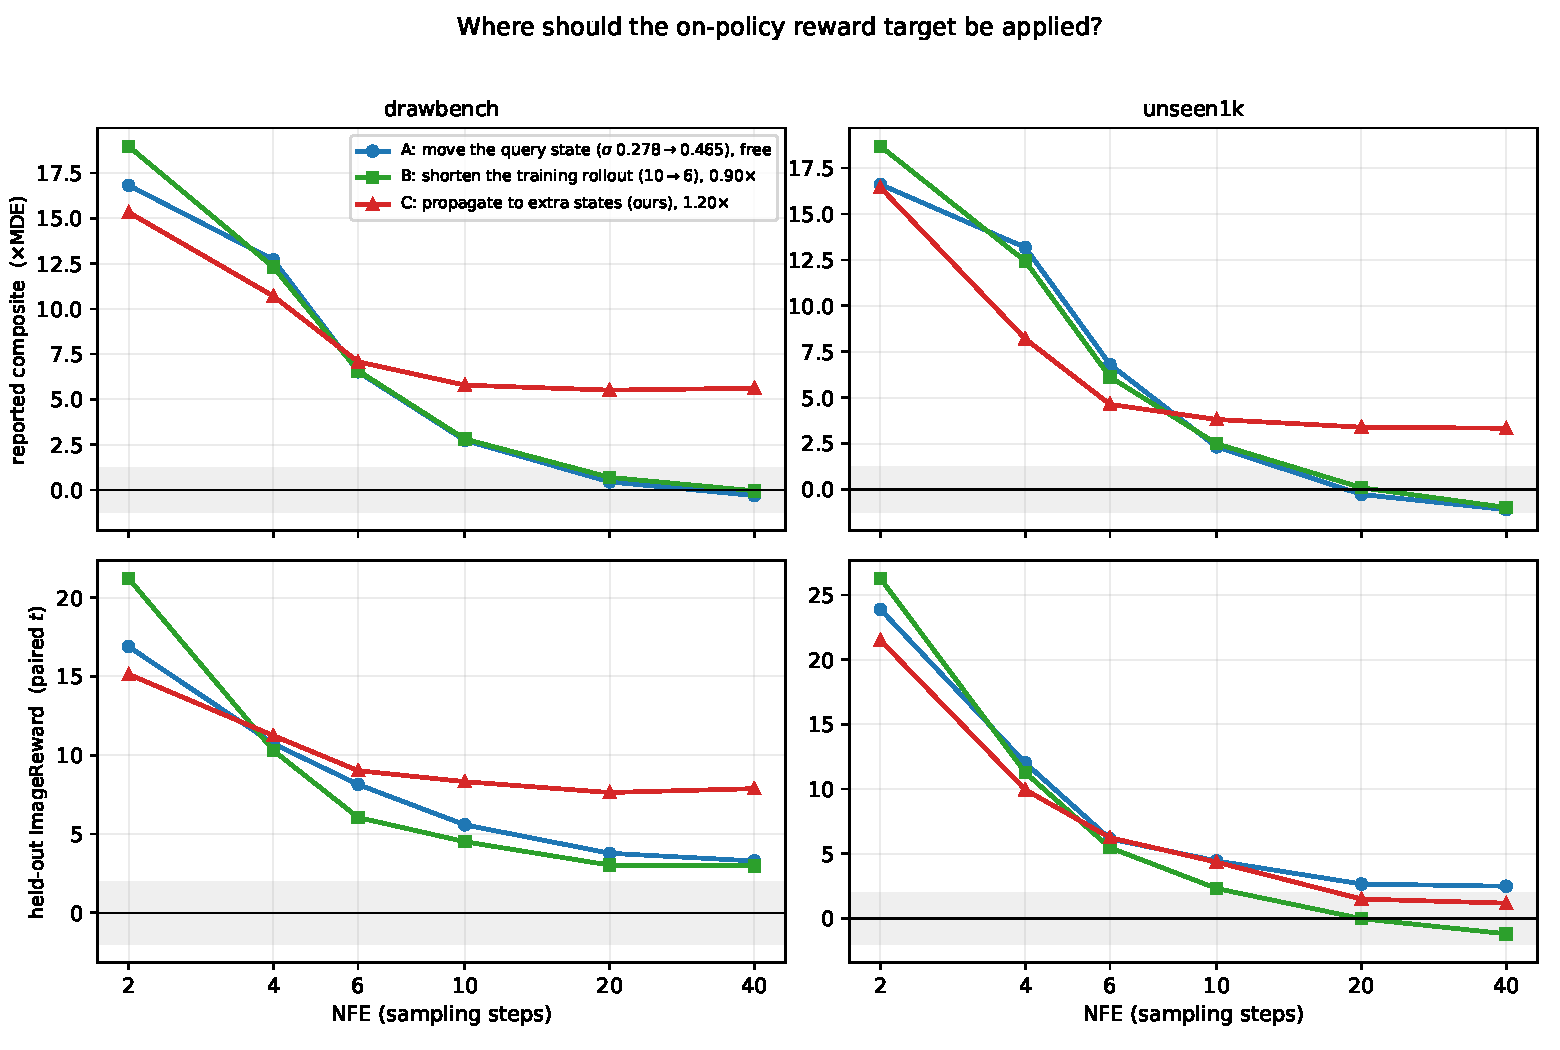
\includegraphics[width=\linewidth]{fig7_where_to_apply.pdf}
\caption{\textbf{Gain versus sampling budget.} Top: reported composite, in MDE. Bottom:
held-out ImageReward, paired $t$. Shaded band is the measured canonical-versus-canonical
floor (top) and $|t|<2$ (bottom). (A) and (B) decay to zero or below by $40$ steps;
(C) flattens at a positive value.}
\label{fig:curves}
\end{figure}

Figure~\ref{fig:curves} shows the full budget sweep. Normalizing each curve by its own
peak, \MSP retains $0.37$ of its peak gain at $40$ steps while the low-step rollout retains
$0.03$ -- the two interventions have different \emph{shapes}, not merely different sizes.

\subsection{Composition}
\label{sec:exp:compose}

% Table 3 — 自动生成。组合与增量。
\begin{table}[t]
\centering
\setlength{\tabcolsep}{4pt}
\caption{\textbf{Composition.} Propagation stacks on top of a shortened rollout.
Top block: each configuration against the canonical baseline. Bottom row: the
\emph{increment} contributed by propagation on top of the shortened rollout.
Units of MDE, win\% in parentheses; $100$ updates, matched hardware and seed.}
\label{tab:compose}
\resizebox{\linewidth}{!}{%
\begin{tabular}{lc cc cc}
\toprule
& & \multicolumn{2}{c}{\textbf{DrawBench}} & \multicolumn{2}{c}{\textbf{Unseen-1k}} \\
\cmidrule(lr){3-4}\cmidrule(lr){5-6}
\textbf{Configuration} & \textbf{Cost} & NFE$=$4 & NFE$=$40 & NFE$=$4 & NFE$=$40 \\
\midrule
(B) shortened rollout & $0.90\times$ & $+12.30$ \scriptsize(91\%) & $-0.05$ \scriptsize(48\%) & $+12.43$ \scriptsize(94\%) & $-0.98$ \scriptsize(43\%) \\
(C) \MSP & $1.20\times$ & $+10.70$ \scriptsize(83\%) & $+5.62$ \scriptsize(71\%) & $+8.20$ \scriptsize(80\%) & $+3.34$ \scriptsize(64\%) \\
\textbf{(B$+$C)} & $\sim\!1.10\times$ & $+16.23$ \scriptsize(93\%) & $+2.26$ \scriptsize(56\%) & $+15.91$ \scriptsize(95\%) & $+1.45$ \scriptsize(54\%) \\
\midrule
\quad increment of (C) over (B) & -- & $+3.93$ \scriptsize(67\%) & $+2.32$ \scriptsize(59\%) & $+3.48$ \scriptsize(70\%) & $+2.43$ \scriptsize(63\%) \\
\bottomrule
\end{tabular}}
\end{table}


\MSP composes with the cheap intervention rather than competing with it
(Table~\ref{tab:compose}). The increment contributed by propagation on top of a $6$-step
rollout is positive in all four cells -- $+3.93$ and $+2.32$ MDE on DrawBench,
$+3.48$ and $+2.43$ on Unseen-1k at $4$ and $40$ steps ($t$ from $+6.8$ to $+13.3$) -- and
it converts (B)'s full-budget loss into a gain. The resulting configuration attains the
largest few-step numbers in the study: $+16.23$ MDE ($92.7\%$ win rate) and $+15.91$ MDE
($95.4\%$). The increment grows with training (from $+3.10/+1.47$ at $50$ updates), which
is the opposite of what an under-training artifact would do.

The two configurations are complementary operating points of the same mechanism. Against
\emph{pure} \MSP, (B$+$C) trades $-3.35$ and $-1.88$ MDE at the full budget for $+5.53$ and
$+7.71$ MDE at $4$ steps -- a favourable exchange whenever inference is the bottleneck,
which is precisely the regime few-step samplers are built for. A practical reading:
\emph{if you will deploy at few steps, use (B$+$C); if one model must serve every budget,
use (C); if you can change only one line, use (A).}

\subsection{Replication and robustness}
\label{sec:exp:robust}

\paragraph{Seeds.} A second random seed, run on different hardware and at a different
world size, and compared against \emph{its own} matched canonical baseline, reproduces the
effect. At $50$ updates all four cells replicate with slightly larger magnitude --
$+8.45$ vs.\ $+7.52$ and $+4.04$ vs.\ $+3.19$ (DrawBench, $4$ and $40$ steps),
$+6.50$ vs.\ $+6.06$ and $+1.69$ vs.\ $+1.22$ (Unseen-1k) -- with a largest seed-to-seed
difference of $0.93$ MDE, below the measured floor. At $100$ updates the two DrawBench
cells give $+9.65$ and $+3.90$ against $+10.70$ and $+5.62$: the same sign, both still
clearing the threshold, with differences of $1.05$ and $1.72$ MDE. The second of those
exceeds the same-configuration floor, but these two runs differ in hardware and world size
as well as in seed, so we read it as agreement in sign and significance rather than in
magnitude.

\paragraph{Training checkpoint.} The few-step gain does not depend on where training is
stopped. A dense checkpoint sweep of the $\mathcal K=\{5,6,7\}$ family member -- the one for
which per-checkpoint canonical controls exist on matched hardware -- is positive at every
point ($20$, $30$, $50$, $80$, $100$ updates: $+8.16$, $+5.43$, $+7.05$, $+9.15$, $+8.48$
MDE on DrawBench; $+7.37$, $+5.38$, $+6.09$, $+7.62$, $+6.47$ on Unseen-1k). The default
$\mathcal K=\{3,6\}$ is measurable at five checkpoints against same-hardware controls. At
$4$ steps it clears the threshold at every one of them -- $+6.66$, $+5.56$, $+7.52$,
$+10.42$, $+10.70$ MDE on DrawBench at $20$, $30$, $50$, $80$ and $100$ updates, and
$+5.95$, $+4.83$, $+6.06$, $+8.19$, $+8.20$ on Unseen-1k -- so over this range the few-step gain
is not an artifact of extended training, and it has essentially plateaued by $80$ updates.
The \emph{full-budget} gain behaves differently across the same range: it grows
($+2.39\!\to\!+5.62$ on DrawBench, $+1.38\!\to\!+3.34$ on Unseen-1k) and only clears the
threshold on both prompt sets at $100$ updates. The two sampling budgets therefore mature at
different rates, and the claim that propagation gains at every sampling budget is one we can
make at $100$ updates, not at $20$ (App.~\ref{app:ckpt}).

\textbf{Both statements are bounded above by $100$ updates.} Trained to the published $300$
instead, the comparison reverses: propagation ends $7.2$ MDE behind at four steps and $9.2$
behind at forty on DrawBench. We report that run in Table~\ref{tab:official} and analyse it
in App.~\ref{app:ckpt}; everything claimed above is at $100$ updates, which is the budget at
which all of our comparisons are matched.

\paragraph{Per-axis.} On DrawBench all four reward axes are positive at all six budgets
and grow monotonically as the budget shrinks. On Unseen-1k the held-out ImageReward is
significant for $\mathrm{NFE}\le10$ and not significant at $20$ and $40$
($t=+1.50,+1.18$); we state this limitation rather than aggregating it away
(App.~\ref{app:peraxis}).

\subsection{Qualitative}
\label{sec:exp:qual}

\begin{figure}[t]
\centering
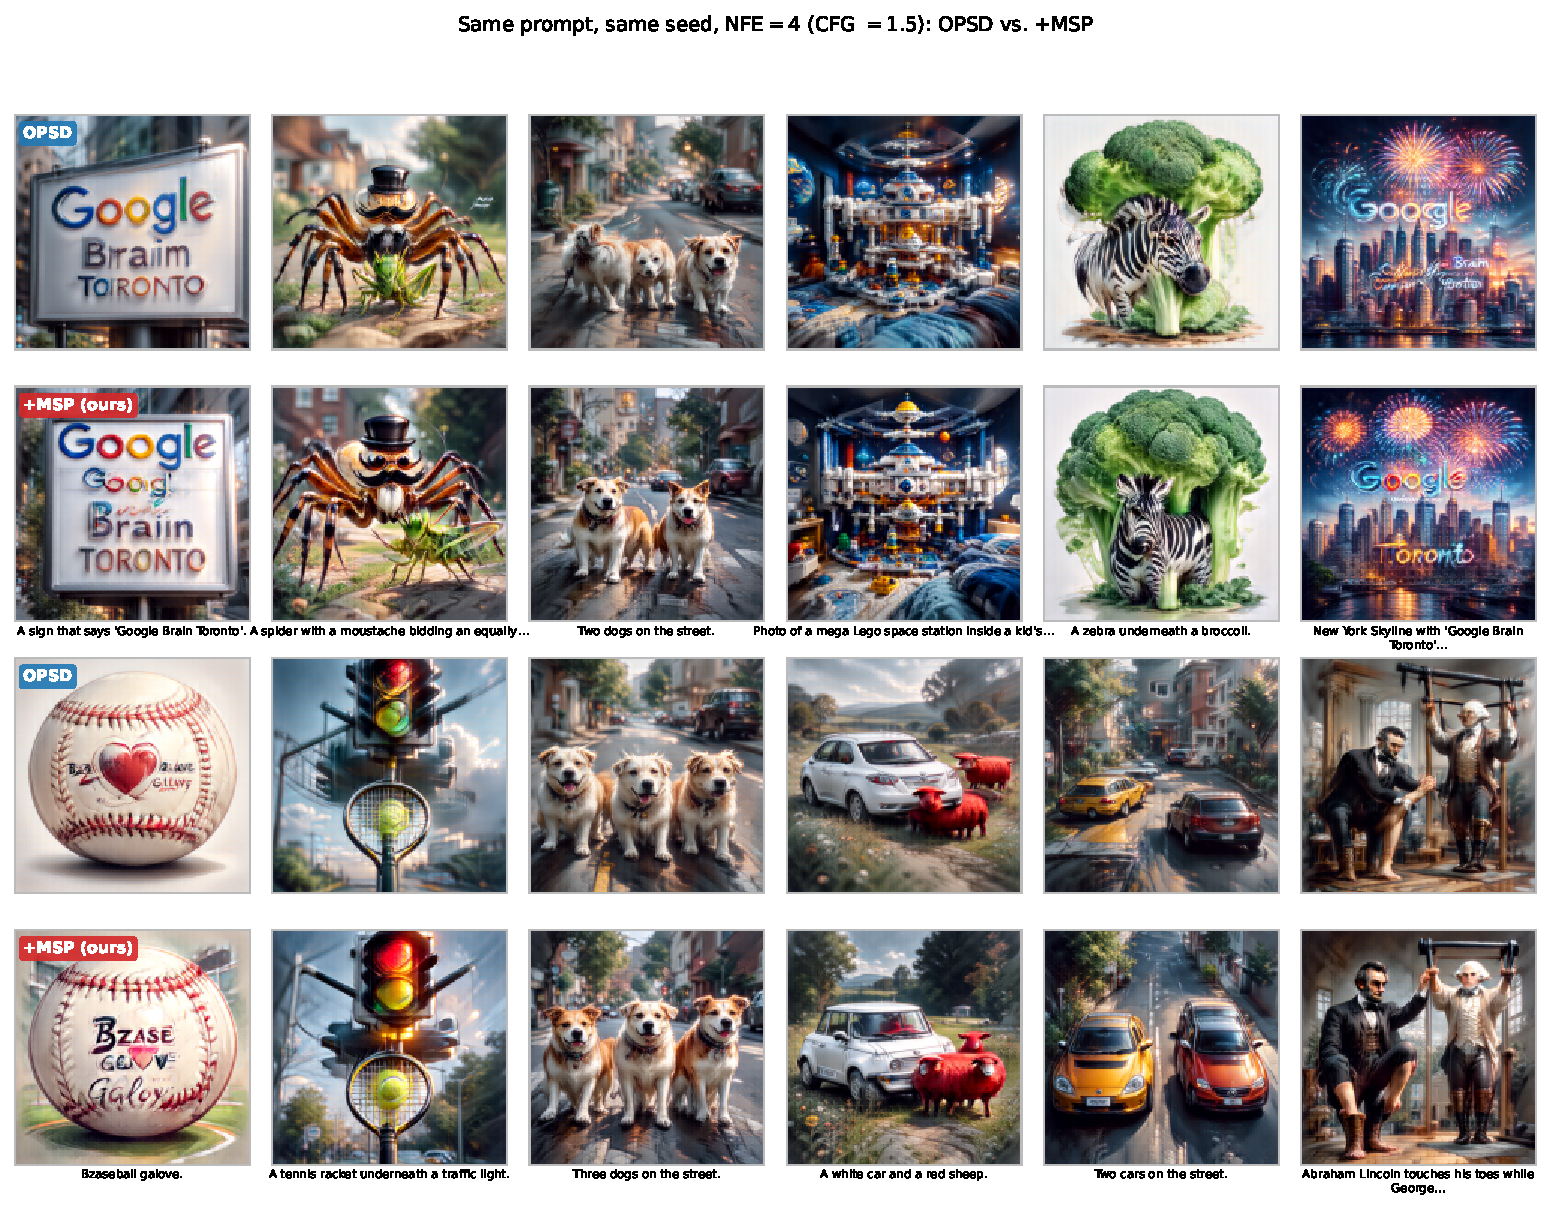
\includegraphics[width=\linewidth]{fig6_qualitative_cfg.pdf}
\caption{\textbf{Four sampling steps, same prompt, same seed; only the model changes.}
\emph{All twelve} prompts selected in advance by a fixed rule (above-median absolute score
under our model, ranked by paired improvement) are shown, with no second pass of manual
filtering; an unselected panel is in App.~\ref{app:qual}. The rule favours prompts whose
differences are checkable by eye rather than by taste: object counts (\emph{two} dogs ---
canonical renders three), spatial relations (the racket \emph{underneath} the traffic
light), and text. Two panels are ties and one (Lincoln) favours canonical; we show them.
These panels are rendered at guidance scale $1.5$ rather than the CFG-free setting used for
every number in this paper, because the CFG-free protocol is a poor \emph{display} setting
at four steps (App.~\ref{app:protocol}); the quantitative protocol is unchanged.}
\label{fig:qual}
\end{figure}
